\documentclass[11pt]{IEEEtran}
\usepackage{endnotes,url,color}
\usepackage{array}
\usepackage[english]{babel}
\usepackage{xspace}
\usepackage{verbatim}
\usepackage[ruled, vlined]{algorithm2e}
\usepackage{amsmath,amssymb}
\usepackage{caption}
\usepackage{natbib}
\usepackage{fancyhdr}
\usepackage[caption=false,font=footnotesize]{subfig}
\usepackage{listings}

 % Add navigation window to pdf
\usepackage{hyperref}
\hypersetup{pdftex,colorlinks=true,allcolors=blue}
\usepackage{hypcap}
\usepackage{xr}

%special fonts
\usepackage{mathpazo} % math & rm
\linespread{1.03}        % Palatino needs more leading (space between lines)

\usepackage{tikz}
\usetikzlibrary{chains,shapes.multipart}

\tikzset{%
  xrightarrow/.style={
    rectangle split,
    anchor=text split west,
    rectangle split parts=2,
    append after command={%
      (\tikzlastnode.text split west) edge[->] (\tikzlastnode.text split east)
    }
  }
}


% -*- root: main.tex -*-

%space left between floats.
\setlength{\floatsep}{4mm}
% space between last top float or first bottom float and the text.
\setlength{\textfloatsep}{2mm}

% space left on top and bottom of an in-text float.
\setlength{\intextsep}{0.5mm}
% space above caption
\setlength{\abovecaptionskip}{2mm}
%space below caption
\setlength{\belowcaptionskip}{0mm}

%% Change figure handling
\renewcommand{\topfraction}{0.9}
\renewcommand{\textfraction}{0.1}
\renewcommand{\floatpagefraction}{1}

%\usepackage[small,compact,noindentafter]{titlesec} 
%\usepackage[compact]{titlesec}

%\titlespacing\section{0pt}{6pt plus 2pt minus 2pt}{2pt plus 2pt minus 2pt}
%\titlespacing\subsection{0pt}{4pt plus 2pt minus 2pt}{2pt plus 1pt minus 1pt}
%\titlespacing{\paragraph}{0pt}{2pt plus 0pt minus 1pt}{1.0ex}

\usepackage[inline]{enumitem}
\setlist{noitemsep,topsep=0pt,parsep=0pt,partopsep=0pt}

\usepackage[subtle]{savetrees}
% \usepackage[moderate]{savetrees}


%%%%%%%%%%%%%%%%%%%%%%%%%%%%%%%%%%%%%%%%%%%%%%%%%%%%%%%%%%%%%%%%%%%%%%
%% mac.tex
%%
%% Umut A. Acar
%% Macros for adaptive computation paper.
%%%%%%%%%%%%%%%%%%%%%%%%%%%%%%%%%%%%%%%%%%%%%%%%%%%%%%%%%%%%%%%%%%%%%%

\newcommand{\readarrow}{\ensuremath{\Longrightarrow}}
\newcommand{\currenttime}{\ttt{currentTime}\xspace}
\newcommand{\tags}[1]{\ensuremath{\mathsf{tags}(#1)}}
\newcommand{\weight}[1]{\ensuremath{\mathsf{weight}(#1)}}
\newcommand{\dist}[2]{\ensuremath{\delta(#1,#2)}}


\newcommand{\cutspace}{\vspace{-4mm}}

\newcommand{\bomb}[1]{\fbox{\mbox{\emph{\bf {#1}}}}}

\newcommand{\myparagraph}[1]{\smallskip \noindent{\bf {#1}.}}
% formatting stuff
\newcommand{\codecolsep}{1ex}



\newcommand{\rlabel}[1]{\hspace*{-1mm}\mbox{\small{\bf ({#1})}}}

\newcommand{\tablerow}{\\[5ex]}
\newcommand{\tableroww}{\\[7ex]}
\newcommand{\tableline}{
\vspace*{2ex}\\
\hline\\ 
\vspace*{2ex}}

% Don't care
\newcommand{\dontcare}{\_
}

%% filter and quicksort stuff
\newcommand{\ncf}[2]{C^{fil}_{\ensuremath{{#1},{#2}}}}
\newcommand{\ncq}[1]{C^{qsort}_{\ensuremath{#1}}}
\newcommand{\nuf}[3]{P^{fil}_{#1,(\ensuremath{{#2},{#3}})}}
\newcommand{\nuq}[2]{P^{qsort}_{(\ensuremath{{#1},{#2}})}}

%% shorthands
\newcommand{\ddg}{{\sc ddg}}
\newcommand{\ncpa}{change-propagation algorithm}
\newcommand{\adg}{{\sc adg}}
\newcommand{\nwrite}{\texttt{write}}
\newcommand{\nread}{\texttt{read}}
\newcommand{\nmodr}{\texttt{mod}}
\newcommand{\ttt}[1]{\texttt{#1}}
\newcommand{\nmodl}{\texttt{modl}}
\newcommand{\nnil}{\ttt{NIL}}
\newcommand{\ncons}[2]{\ttt{CONS({\ensuremath{#1},\ensuremath{#2}})}}
\newcommand{\nfilter}{\texttt{filter}}
\newcommand{\nfilterp}{\texttt{filter'}}
\newcommand{\naqsort}{\texttt{qsort'}}
\newcommand{\nqsort}{\texttt{qsort}}
\newcommand{\nqsortp}{\texttt{qsort'}}
\newcommand{\nnewMod}{\texttt{newMod}}
\newcommand{\nchange}{\texttt{change}}
\newcommand{\npropagate}{\texttt{propagate}}
\newcommand{\ndest}{\texttt{d}}
\newcommand{\ninit}{\texttt{init}}



%% Comment sth out. 
\newcommand{\out}[1] {}
\newcommand{\sthat}{\ensuremath{~|~}}

%% definitions
\newcommand{\defi}[1]{{\bfseries\itshape #1}}


% Code listings.
\newcounter{codeLineCntr}
\newcommand{\codeLine}
 {\refstepcounter{codeLineCntr}{\thecodeLineCntr}}
\newcommand{\codeLineL}[1]
 {\refstepcounter{codeLineCntr}\label{#1}{\thecodeLineCntr}}
\newcommand{\codeLineNN}{} %% NN = No-Number (and no change to counter)

\newenvironment{codeListing}
 {\setcounter{codeLineCntr}{0}
%  \fontsize{10}{12}
 % the first one is width the second is height
 \fontsize{9}{11}
  \fontsize{8}{8}
  \vspace{-.1in}
  \ttfamily\begin{tabbing}}
  {\end{tabbing}
   \vspace{-.1in}}

\newenvironment{codeListing8}
 {\setcounter{codeLineCntr}{0}
%  \fontsize{8}{10}
  \fontsize{8}{8}
  \vspace{-.1in}
  \ttfamily
  \begin{tabbing}}
 {\end{tabbing}
 \vspace{-.1in}
}

\newenvironment{codeListing8h}
 {\setcounter{codeLineCntr}{0}
  \fontsize{8.5}{10.5}
  \vspace{-.1in}
  \ttfamily
  \begin{tabbing}}
 {\end{tabbing}
 \vspace{-.1in}
}


\newenvironment{codeListing9}
 {\setcounter{codeLineCntr}{0}
  \fontsize{9}{11}
  \vspace{-.1in}
  \ttfamily
  \begin{tabbing}}
 {\end{tabbing}
 \vspace{-.1in}
}

\newenvironment{codeListing10}
 {\setcounter{codeLineCntr}{0}
  \fontsize{10}{12}
  \vspace{-.1in}
  \ttfamily
  \begin{tabbing}}
 {\end{tabbing}
 \vspace{-.1in}
}


\newenvironment{codeListingNormal}
 {\setcounter{codeLineCntr}{0}
  \vspace{-.1in}
  \ttfamily
  \begin{tabbing}}
 {\end{tabbing}
 \vspace{-.1in}
}

\newcommand{\codeFrame}[1]
{\begin{center}\fbox{\parbox[t]{\columnwidth}{#1}}\end{center}
% \vspace*{-.15in}
}

\newcommand{\halfBox}[1]
{\begin{center}\fbox{\parbox[t]{\columnwidth}{#1}}\end{center}
% \vspace*{-.15in}
}

\newcommand{\fullBox}[1]
{\begin{center}\fbox{\parbox[t]{\textwidth}{#1}}\end{center}
% \vspace*{-.15in}
}

%%Note this is redefined in local-mac.tex for each paper.
\newcommand{\fixedCodeFrame}[1]
{
\begin{center}
\fbox{
\parbox[t]{0.9\columnwidth}{
#1
}
}\end{center}
}

% Footnote commands.
\newcommand{\footnotenonumber}[1]{{\def\thempfn{}\footnotetext{#1}}}

% Margin notes - use \notesfalse to turn off notes.
\setlength{\marginparwidth}{0.6in}
\reversemarginpar
\newif\ifnotes
\notestrue
\newcommand{\longnote}[1]{
  \ifnotes
    {\medskip\noindent Note:\marginpar[\hfill$\Longrightarrow$]
      {$\Longleftarrow$}{#1}\medskip}
  \fi}
\newcommand{\note}[1]{
  \ifnotes
    {\marginpar{\raggedright{\tiny #1}}}
  \fi}
\newcommand{\notered}[1]{\ifnotes
    {\marginpar{\raggedright{\tiny
          {\sf\color{red} #1}}}}
    \fi}


% Stuff not wanted.
\newcommand{\punt}[1]{}

% Sectioning commands.
\newcommand{\subsec}[1]{\subsection{\boldmath #1 \unboldmath}}
\newcommand{\subheading}[1]{\subsubsection*{#1}}
\newcommand{\subsubheading}[1]{\paragraph*{#1}}

% Reference shorthands.
\newcommand{\spref}[1]{Modified-Store Property~\ref{sp:#1}}
\newcommand{\prefs}[2]{Properties~\ref{p:#1} and~\ref{p:#2}}
\newcommand{\pref}[1]{Property~\ref{p:#1}}


\newcommand{\partref}[1]{Part~\ref{part:#1}}
\newcommand{\chref}[1]{Chapter~\ref{ch:#1}}
\newcommand{\chreftwo}[2]{Chapters \ref{ch:#1} and~\ref{ch:#2}}
\newcommand{\chrefthree}[3]{Chapters \ref{ch:#1}, and~\ref{ch:#2}, and~\ref{ch:#3}}
\newcommand{\secref}[1]{Section~\ref{sec:#1}}
\newcommand{\subsecref}[1]{Subsection~\ref{subsec:#1}}
\newcommand{\secreftwo}[2]{Sections \ref{sec:#1} and~\ref{sec:#2}}
\newcommand{\secrefthree}[3]{Sections \ref{sec:#1},~\ref{sec:#2},~and~\ref{sec:#3}}
\newcommand{\appref}[1]{Appendix~\ref{app:#1}}
\newcommand{\figref}[1]{Figure~\ref{fig:#1}}
\newcommand{\figreftwo}[2]{Figures \ref{fig:#1} and~\ref{fig:#2}}
\newcommand{\figrefthree}[3]{Figures \ref{fig:#1}, \ref{fig:#2} and~\ref{fig:#3}}
\newcommand{\figreffour}[4]{Figures \ref{fig:#1},~\ref{fig:#2},~\ref{fig:#3}~and~\ref{fig:#4}}
\newcommand{\figpageref}[1]{page~\pageref{fig:#1}}
\newcommand{\tabref}[1]{Table~\ref{tab:#1}}
\newcommand{\tabreftwo}[2]{Tables~\ref{tab:#1} and~\ref{tab:#1}}

\newcommand{\stref}[1]{step~\ref{step:#1}}
\newcommand{\caseref}[1]{case~\ref{case:#1}}
\newcommand{\lineref}[1]{line~\ref{line:#1}}
\newcommand{\linereftwo}[2]{lines \ref{line:#1} and~\ref{line:#2}}
\newcommand{\linerefthree}[3]{lines \ref{line:#1},~\ref{line:#2},~and~\ref{line:#3}}
\newcommand{\linerefrange}[2]{lines \ref{line:#1} through~\ref{line:#2}}
\newcommand{\thmref}[1]{Theorem~\ref{thm:#1}}
\newcommand{\thmreftwo}[2]{Theorems \ref{thm:#1} and~\ref{thm:#2}}
\newcommand{\thmrefthree}[3]{Theorems \ref{thm:#1}, \ref{thm:#2} and~\ref{thm:#3}}
\newcommand{\thmpageref}[1]{page~\pageref{thm:#1}}
\newcommand{\lemref}[1]{Lemma~\ref{lem:#1}}
\newcommand{\lemreftwo}[2]{Lemmas \ref{lem:#1} and~\ref{lem:#2}}
\newcommand{\lemrefthree}[3]{Lemmas \ref{lem:#1},~\ref{lem:#2},~and~\ref{lem:#3}}
\newcommand{\lempageref}[1]{page~\pageref{lem:#1}}
\newcommand{\corref}[1]{Corollary~\ref{cor:#1}}
\newcommand{\defref}[1]{Definition~\ref{def:#1}}
\newcommand{\defreftwo}[2]{Definitions \ref{def:#1} and~\ref{def:#2}}
\newcommand{\defpageref}[1]{page~\pageref{def:#1}}
\renewcommand{\eqref}[1]{Equation~(\ref{eq:#1})}
\newcommand{\eqreftwo}[2]{Equations (\ref{eq:#1}) and~(\ref{eq:#2})}
\newcommand{\eqpageref}[1]{page~\pageref{eq:#1}}
\newcommand{\ineqref}[1]{Inequality~(\ref{ineq:#1})}
\newcommand{\ineqreftwo}[2]{Inequalities (\ref{ineq:#1}) and~(\ref{ineq:#2})}
\newcommand{\ineqpageref}[1]{page~\pageref{ineq:#1}}
\newcommand{\itemref}[1]{Item~\ref{item:#1}}
\newcommand{\itemreftwo}[2]{Item~\ref{item:#1} and~\ref{item:#2}}

% Useful shorthands.
\newcommand{\abs}[1]{\left| #1\right|}
\newcommand{\card}[1]{\left| #1\right|}
\newcommand{\norm}[1]{\left\| #1\right\|}
\newcommand{\floor}[1]{\left\lfloor #1 \right\rfloor}
\newcommand{\ceil}[1]{\left\lceil #1 \right\rceil}
  \renewcommand{\choose}[2]{{{#1}\atopwithdelims(){#2}}}
\newcommand{\ang}[1]{\langle#1\rangle}
\newcommand{\paren}[1]{\left(#1\right)}
\newcommand{\prob}[1]{\Pr\left\{ #1 \right\}}
\newcommand{\expect}[1]{\mathrm{E}\left[ #1 \right]}
\newcommand{\expectsq}[1]{\mathrm{E}^2\left[ #1 \right]}
\newcommand{\variance}[1]{\mathrm{Var}\left[ #1 \right]}
\newcommand{\twodots}{\mathinner{\ldotp\ldotp}}

% Standard number sets.
\newcommand{\reals}{{\mathrm{I}\!\mathrm{R}}}
\newcommand{\integers}{\mathbf{Z}}
\newcommand{\naturals}{{\mathrm{I}\!\mathrm{N}}}
\newcommand{\rationals}{\mathbf{Q}}
\newcommand{\complex}{\mathbf{C}}

% Special styles.
\newcommand{\proc}[1]{\ifmmode\mbox{\textsc{#1}}\else\textsc{#1}\fi}
\newcommand{\procdecl}[1]{
  \proc{#1}\vrule width0pt height0pt depth 7pt \relax}
  \newcommand{\func}[1]{\ifmmode\mathrm{#1}\else\textrm{#1}fi} %
%  Multiple cases.  
\renewcommand{\cases}[1]{\left\{
  \begin{array}{ll}#1\end{array}\right.}
  \newcommand{\cif}[1]{\mbox{if $#1$}} 

%% spacing hacks
\newcommand{\longpage}{\enlargethispage{\baselineskip}}
\newcommand{\shortpage}{\enlargethispage{-\baselineskip}}



%% Notes, todos, and remarks
\newcounter{remark}[section]

\newcommand{\myremark}[3]{
\refstepcounter{remark}
\[
\left\{
\sf 
\parbox{\columnwidth}{
{\bf {#1}'s remark~\theremark:} 
{#3}
}
\right\}
\]
%\marginpar{\bf {#2}.~\theremark}
}


% - - - - - - - - - - - - - - - - - - - - - - - - - - - - - - - - - - - - - - - - - - - - 
% For amsthm package:

%\theoremstyle{plain}
%\newtheorem{thm}{Theorem}[section]
%% \newtheorem{lem}[thm]{Lemma}
%% \newtheorem{prop}[thm]{Proposition}
%% \newtheorem*{cor}{Corollary}

%% \theoremstyle{definition}
%% \newtheorem{defn}{Definition}[section]
%% \newtheorem{conj}{Conjecture}[section]
%% \newtheorem{falseconj}{False~Conjecture}[section]
%% \newtheorem{exmp}{Example}[section]

%% \theoremstyle{remark}
%% \newtheorem*{rem}{Remark}
%% %\newtheorem*{note}{Note}
%% \newtheorem{case}{Case}


\newcommand{\uremark}[1]{\myremark{Umut}{U}{#1}}
\newcommand{\ur}[1]{\uremark{#1}}
\newcommand{\rremark}[1]{\myremark{Ruy}{R}{#1}}
\newcommand{\mremark}[1]{\myremark{Matthew}{M}{#1}}
\newcommand{\todoremark}[1]{\myremark{TODO}{TODO}{#1}}
%\newcommand{\todo}[1]{\myremark{TODO}{TODO}{#1}}
\newcommand{\todo}[1]{{\bf{[TODO:{#1}]}}}

%%

%% 
%% Functions
\newcommand{\timeOfTask}[1]{\ensuremath{t_T {#1} }}
\newcommand{\timeRead}[1]{\ensuremath{t_R {#1} }}
\newcommand{\timeWrite}[1]{\ensuremath{t_W {#1} }}


%% sets
\newcommand{\setFresh}{\mathcal{F}}
\newcommand{\setReused}{\mathcal{R}}


%% times
\newcommand{\timeHash}{\ensuremath{t_h}\xspace}
\newcommand{\timeMessage}{\ensuremath{t_m}\xspace}
\newcommand{\timeMemo}{\ensuremath{t_{memo}}\xspace}
\newcommand{\ninput}{\ensuremath{n_i}\xspace}
\newcommand{\noutput}{\ensuremath{n_O}\xspace}
\newcommand{\nmap}{\ensuremath{N_M}\xspace}
\newcommand{\nred}{\ensuremath{N_R}\xspace}
\newcommand{\ncon}{\ensuremath{N_C}\xspace}

\newcommand{\nkeysetmap}{\ensuremath{n_{mk}}}
\newcommand{\nkeyvaluemap}{\ensuremath{n_{m}}}
\newcommand{\nconAppend}{\ensuremath{H_{CA}}\xspace}
\newcommand{\nconFix}{\ensuremath{H_{CF}}\xspace}
\newcommand{\nconVariable}{\ensuremath{H_{CV}}\xspace}

%% numbers
\newcommand{\numberTasks}{\ensuremath{n_t}}
\newcommand{\inputSize}{\ensuremath{s_i}}
\newcommand{\avgChunkSize}{\ensuremath{s_c}}
\newcommand{\keyset}{\ensuremath{K}}


%% sizes
\newcommand{\sizeReducers}{\ensuremath{m_r}}



\newcommand{\myfontsize}{\fontsize{7}{9}\selectfont}

\newcommand{\myreffontsize}{\fontsize{8.5}{9.5}\selectfont}

\begin{document}

\author{
\IEEEauthorblockN{J{\"o}rg Thalheim}\\
\IEEEauthorblockA{TU Dresden}\\
}

\title{\huge The Impact of TCP's Initial Congestion Window}
\maketitle
\begin{abstract}
The initial congestion window is an important parameter of the TCP slow start
algorithm. It defines the upper limit of outstanding bytes a sender assumes at
the beginning of new connection.

The current standard RFC3390~\cite{rfc3390} from 2002 specifies a window of four
segments (over 4KB). Large-scale experiments~\cite{36640} by Google from 2010
have shown that an increase of the initial congestion window improves the
overall performance of web servers without a negative impact on the network
stability. In their research they measured transmission time for web requests to
their services. These only transmit a small amount of data and take a short
time. Therefor the tcp connections do not live long enough to build up a
congestion window big enough to make efficient use of the available bandwidth.
Driven by these results, the experimental standard RFC6928~\cite{rfc6928} was
made to propose an increase of the TCP's Initial Window to 10 segments.

In this paper the effect of different TCP's Initial Windows on user latency is
evaluated in a controlled environment simulating various network condition with
the use of Mininet~\cite{mininet}.

First we present the TCP congestion control mechanisms and how certain network
conditions influence throughput and transmission time. Then we show our
measurement methodology. After that we will evaluate our results and discuss the
outcomes.
\vspace{-4mm}
\end{abstract}


\section{Introduction}
\label{sec:introduction}

The Transmission Control Protcol, short TCP, is most popular communication
protcol on the Internet. To make it scaleable and adaptive to the current
condition of network without overloading it, congestion control mechanism are
used. Part of these algorithm is TCP slow start as decribed in
RFC5681~\cite{rfc5681}.

The TCP slow algoritm limits the number of bytes it sends on a new tcp
connection before waiting for an acknowledgement. On every acknowleged packet
the sender increases the window size by one segment until the Slow-start
threshold (\emph{ssthres}) is reached  or the receiver advertises a lower
receiver window (\emph{rwnd}) in its tcp header. The exponential grow of the
window every roundtrip will be also stopped if TCP detects packet loss. This
could be indicated by either a duplicate acknowlegdment of the receiver or a
timeout. Depending on the congestion algorithm in use the sender will then
behave differently. TCP Reno~\cite{rfc2581} is currently the most widely
deployed. On timeout it will reduce the congestion window to 1. If it receives
an acknowledgment for the same packet three times in a row, it will half
congestion window. The new Slow-Start threshold will be set to the
current window. The sender assumes that the packet after the one, it received
duplicate ACKs for, got lost and will perform a retransmit (also known as Fast
Retransmit). It then enters a phase called Fast Recovery. In this phase the
sender will increase the congestion window only one segment per round trip,
which is equivalent to linear growth.

Other congestion algorithm have slightly different behavior on how they behave
when congestion is detected. In picture~\ref{fig:cwnd_tcp_algos} the grow of tcp
congestion windows for different tcp congestion algorithm is depicted. An
Assumption that most tcp congestion algorithm make is that the majority packet
loss in the network occurs because overloading the network at bottlenecks rather
thank faulty transmission. Router in the network have a limited queue they fill
up before they begin to drop IP packets. Bottlenecks in the network occur
because links have assymmetric bandwith or usage.

\begin{figure*}[ht]
\footnotesize
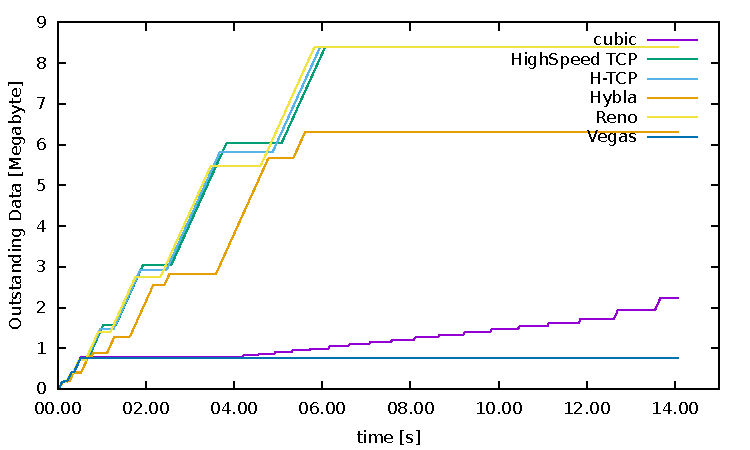
\includegraphics[scale=0.8]{figure/b2a_owin.pdf}
\caption{Congestion window grow over time for different tcp congestion
algorithm for a single connection over 10mbit link with a forwarding delay of
10ms}
\label{fig:cwnd_tcp_algos}
\end{figure*}

The initial congestion window therefor defines the upper limit of bytes a sender assumes at
the beginning.

\section{Measurement Setup}
\label{sec:measurement_setup}

To research the influence of different initial window size on TCP and the
network, we chose the network virtualization framework Mininet~\cite{mininet}.
Mininet exploits existing os virtualization and resource management features of
the Linux kernel, namely Network namespaces~\cite{network_namespaces} and
Cgroups~\cite{cgroups}, to simulate multiple networks and peers on a single
host. Because no virtual machines are involved and Linux can make advantage of
zero-copy mechanism, the overhead of these Network namespaces is low. It can
easily simulate 10GbE-Networks using commodity PC-Hardware. Mininet also
integrates other features such as traffic control and OpenFlow, so one can build
arbitrary network topologies and conditions. To create and configure networks
Mininet exposes a Python API and allow to interact with network namespaces at
runtime by giving shell access.

\newcommand{\FixedScale}{0.7}

\begin{figure*}
\begin{tikzpicture}[
  start chain=going right,
  diagram item/.style={
    on chain,
    join
  },
  node distance=1cm and 3cm,
  scale=0.8, every node/.style={transform shape}
]

\node [
  diagram item,
  label=below:{Server (Nginx)}
] (server) {
\includegraphics[scale=\FixedScale]{figure/server_w_pc_router}};

\node [
  diagram item,
  label=center:{Internet}
] (internet) {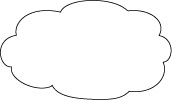
\includegraphics[scale=\FixedScale]{figure/cloud}};

\node [
  diagram item,
  label=below:Modem/Router
] (router) {
\includegraphics[scale=\FixedScale]{figure/cable_modem}};

\node [
  diagram item,
  label=below:{Client (cURL)}
] (client) {
\includegraphics[scale=\FixedScale]{figure/pc}};

\draw (server)   -- (internet);
\draw (internet) -- (router) node[pos=0.62,text width=3cm] {BW: variable,\\Delay: variable};
\draw (router)   -- (client) node[pos=0.62,text width=3cm] {BW: 1Gbps,\\Delay: 1ms};
\end{tikzpicture}
\caption{Network Topology simulated using Mininet}
\end{figure*}


All measurement code and code related to mininet can be found in the following
repository: \url{https://github.com/Mic92/acto15-tcpicw}. For our network
topology we have chosen a setup as depicted in figure~\ref{fig:topology}. Both
client and server are represented by host. They are connected via virtual
ethnernet pairs to a software bridge, which represents our router. The veth pair
of the server stands for the Uplink the client has over the internet to our
server. The other one is the local area network, where both client and router
are included. To limit the bandwith and set a forwarding delay, we applied
policies using Linux's Traffic Control~\cite{tc}. The Link between client and
router was constantly limited to 1GB with a forwarding delay of 1ms. The
assumption made in our topology was, that the bottleneck often is the uplink of
the client. The TCP receive/send window was globally with to be large enough to
fit even the largest requests made during this experiment. The relevant sysctl
configuration is the following.

\begin{lstlisting}
# /etc/sysctl.conf
net.ipv4.tcp_window_scaling = 1

net.core.wmem_max = 16777216
net.ipv4.tcp_wmem = 10240 87380 16777216
net.ipv4.tcp_rmem = 10240 87380 16777216
\end{lstlisting}

As scheduling algorithm we used HFSC. As TCP congestion algorithm
Cubic~\cite{cubic} was in use, which is the default on Linux. The router was
configured to have a queue length of 1000 packets. As application of TCP we
decied to use HTTP. Therefor we started Nginx~\cite{nginx} in version 1.8.0 on
the the server and set it up to serve static files:

\begin{lstlisting}
# nginx.conf
pid nginx.pid;
user root;
error_log stderr;
events { worker_connections  1024; }
http { server {
    listen 80;
    location / { root www; }
} }
\end{lstlisting}

On the client, we use cURL~\cite{curl} to issue HTTP requests. To match up
better with real browsers in term of request size, the HTTP header, a Google
Chrome browser would do, was chosen.

The following test parameter were used:

\begin{itemize}
  \item initial window size (on both links) in segments: 3, 4, 5, 6, 7, 8, 9, 10, 12, 14, 18, 24, 32, 40, 60
  \item uplink forwarding delay in ms: 1, 5, 10, 50, 100, 300
  \item uplink bandwith in mbit/s: 1, 2, 5, 10, 100
  \item requests size in kb (only payload, not http): 1, 2, 4, 16, 32, 64, 128, 256, 512, 1024, 2048, 4096, 8192, 16384
\end{itemize}

After each run we the network environment was recreated. The initial window size
was applied by setting \emph{initcwnd} route attributes with iproute2. The total
request time was reported on receiver site by curl.


\section{Measurement Setup}
\label{sec:measurement_setup}

To research the influence of different initial window size on TCP and the
network, we chose the network virtualization framework Mininet~\cite{mininet}.
Mininet exploits existing os virtualization and resource management features of
the Linux kernel, namely Network namespaces~\cite{network_namespaces} and
Cgroups~\cite{cgroups}, to simulate multiple networks and peers on a single
host. Because no virtual machines are involved and Linux can make advantage of
zero-copy mechanism, the overhead of these Network namespaces is low. It can
easily simulate 10GbE-Networks using commodity PC-Hardware. Mininet also
integrates other features such as traffic control and OpenFlow, so one can build
arbitrary network topologies and conditions. To create and configure networks
Mininet exposes a Python API and allow to interact with network namespaces at
runtime by giving shell access.

\newcommand{\FixedScale}{0.7}

\begin{figure*}
\begin{tikzpicture}[
  start chain=going right,
  diagram item/.style={
    on chain,
    join
  },
  node distance=1cm and 3cm,
  scale=0.8, every node/.style={transform shape}
]

\node [
  diagram item,
  label=below:{Server (Nginx)}
] (server) {
\includegraphics[scale=\FixedScale]{figure/server_w_pc_router}};

\node [
  diagram item,
  label=center:{Internet}
] (internet) {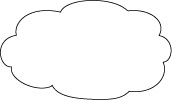
\includegraphics[scale=\FixedScale]{figure/cloud}};

\node [
  diagram item,
  label=below:Modem/Router
] (router) {
\includegraphics[scale=\FixedScale]{figure/cable_modem}};

\node [
  diagram item,
  label=below:{Client (cURL)}
] (client) {
\includegraphics[scale=\FixedScale]{figure/pc}};

\draw (server)   -- (internet);
\draw (internet) -- (router) node[pos=0.62,text width=3cm] {BW: variable,\\Delay: variable};
\draw (router)   -- (client) node[pos=0.62,text width=3cm] {BW: 1Gbps,\\Delay: 1ms};
\end{tikzpicture}
\caption{Network Topology simulated using Mininet}
\end{figure*}



\section{Discussion}
\label{sec:discussion}

The result of this experiment shows possible gains by increasing the initial
congestion window for shorter bursty connection. However the topology selected
for testing is rather simple compared to the internet. It does not take
congested overloaded networks into account. High \emph{initcwnd} might hurt
network stability in this case, because congestion is perceived later.
In our network the bandwidth on all link was symmetric. Often client
networks are often asymmetric connected to the internet.
In case of downlink oriented traffic clients only need a fraction of uplink
speed to acknowledge packages. However in some cases if upload capacity is shared
with other flows, queues are filled up with and causes long delays. This phenomenon
is called buffer bloat~\cite{rfc970}. Longer congestion windows will have a
positive effect in case the downlink is not congested.

%# Testsetup
%
%## Grenzen der Simulation:
%- Nur den Linux-TCP Stack und dessen Standardeinstellungen betrachtet
%
%- bw = (cwnd * mtu) / rtt

\begin{figure*}[ht]
\begin{center}
\footnotesize
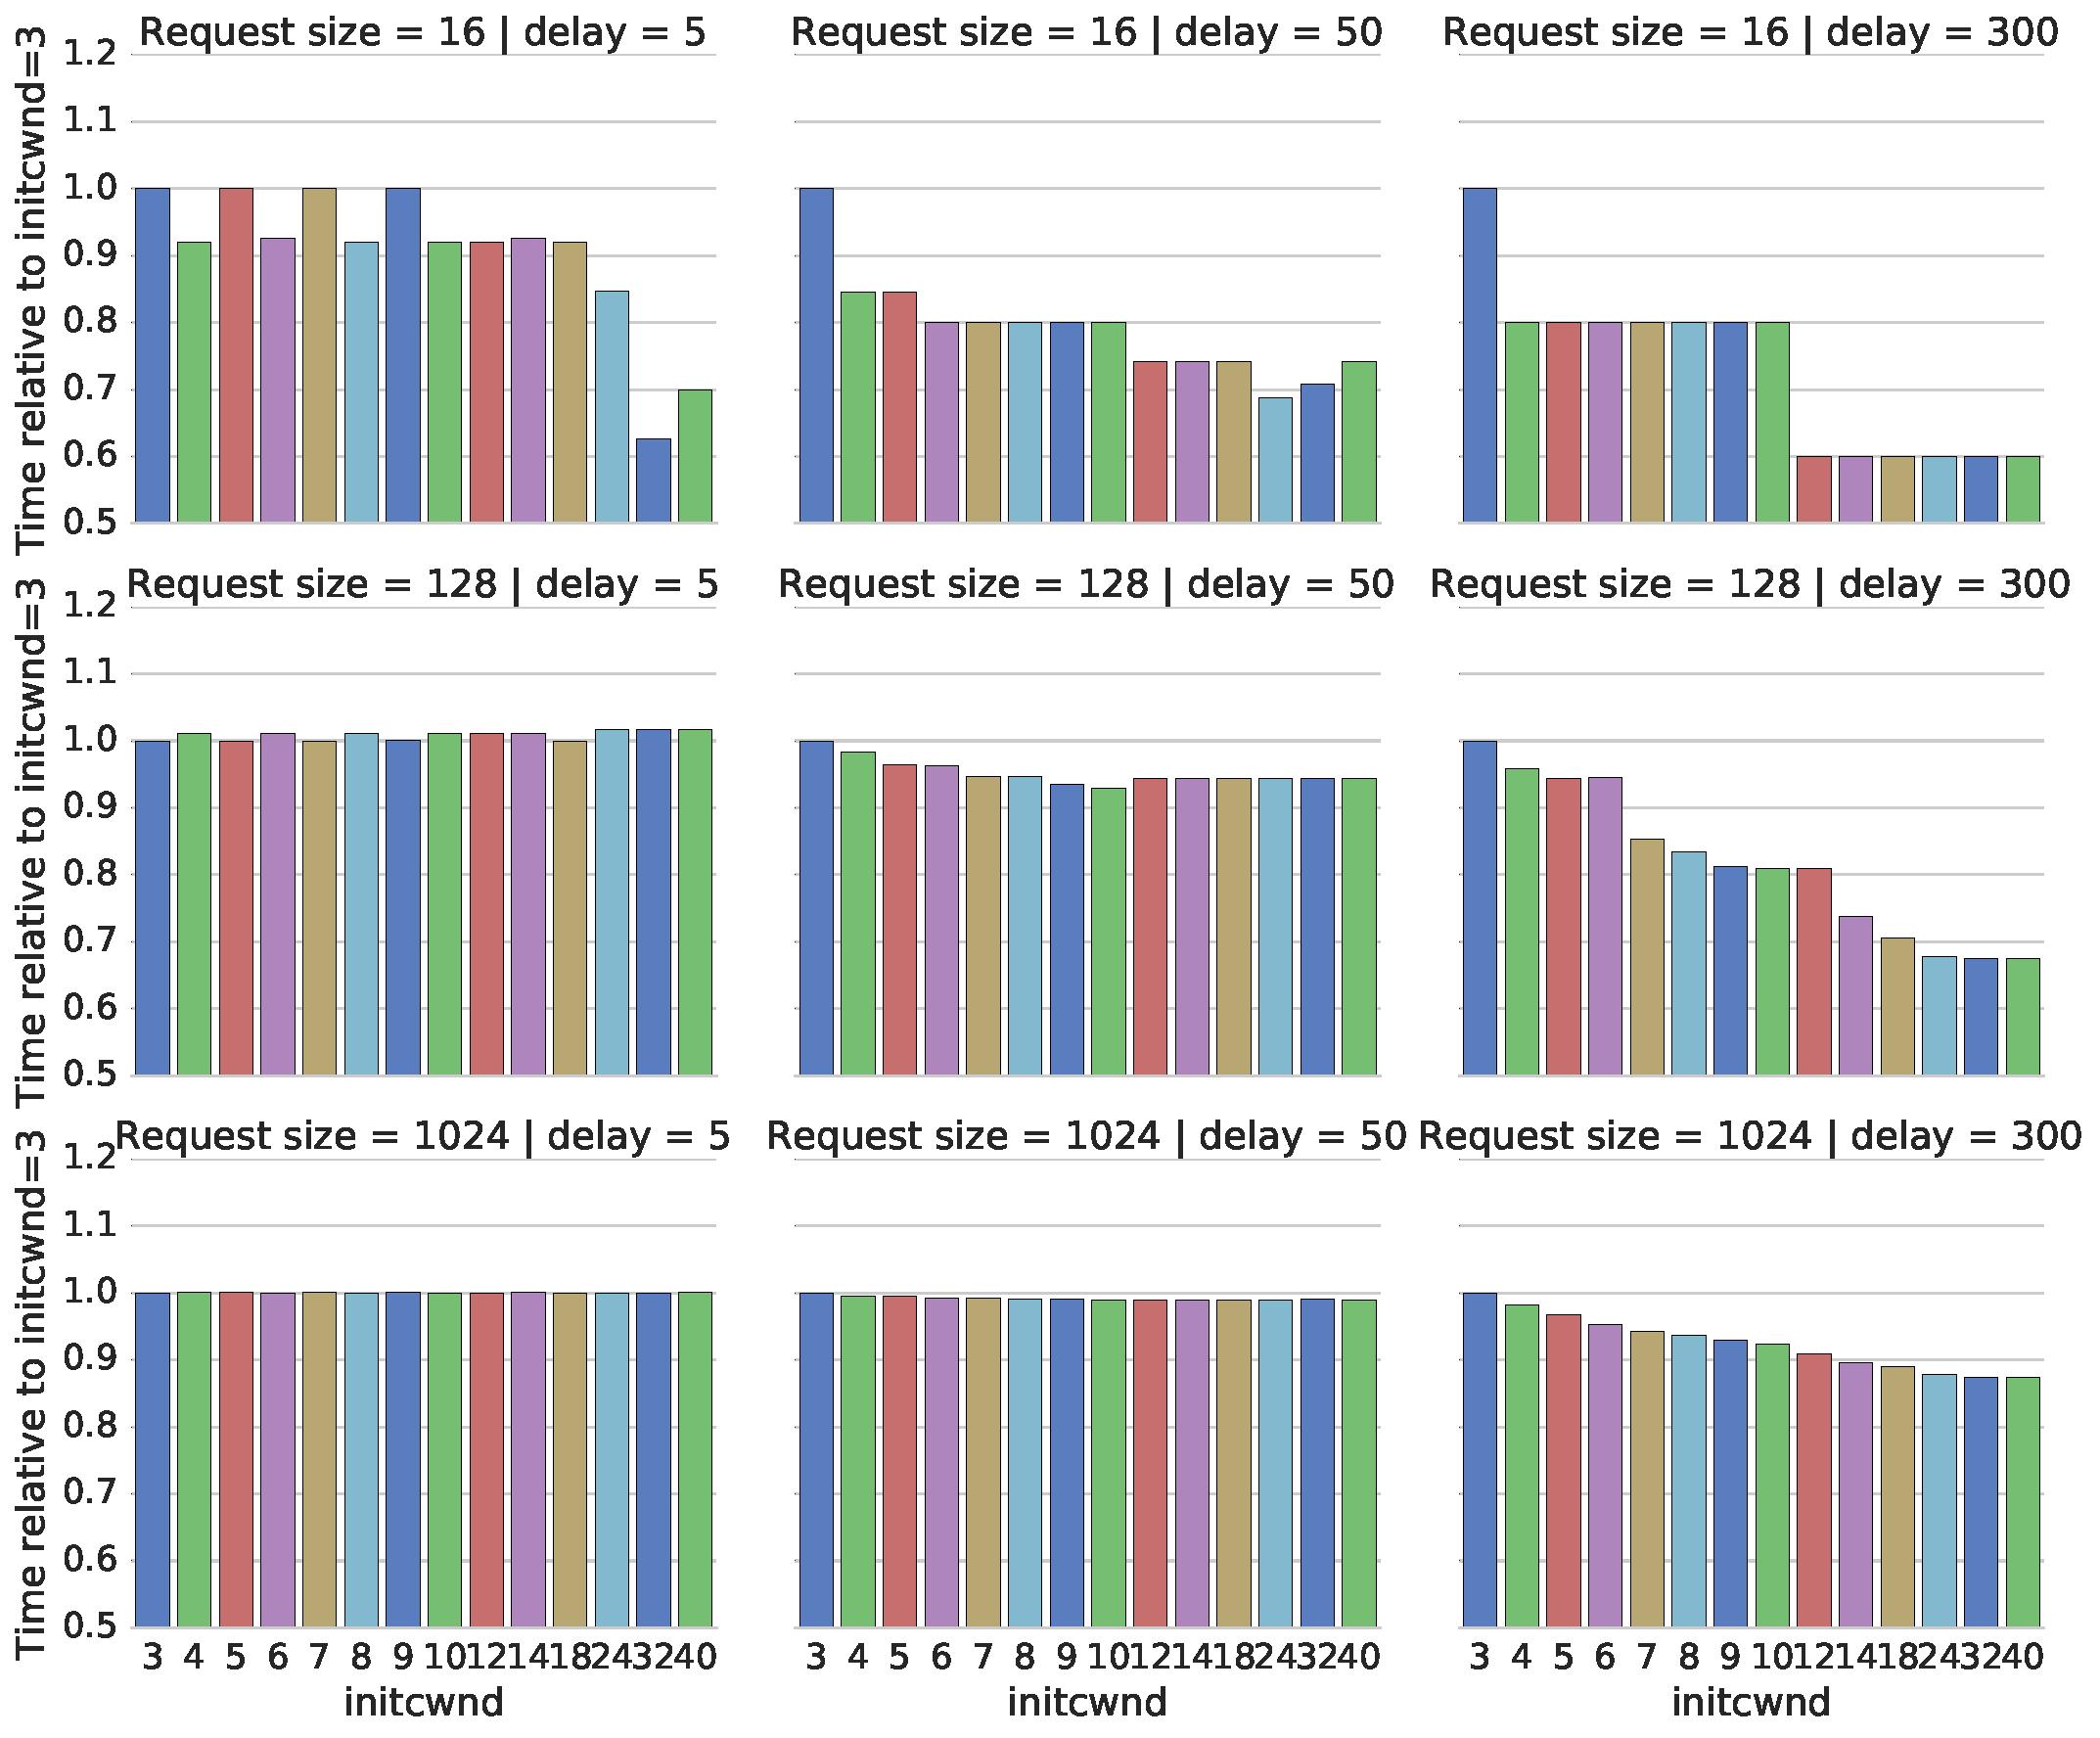
\includegraphics[scale=0.35]{figure/bandwidth-1mb}
\caption{Request time relative to a window of 3 segments with a bandwidth of
1MBps with varying forwarding delay [seconds] and varying request size [kiB]}
\label{fig:bandwith-1mb}
\end{center}
\end{figure*}

\begin{figure*}[ht]
\begin{center}
\footnotesize
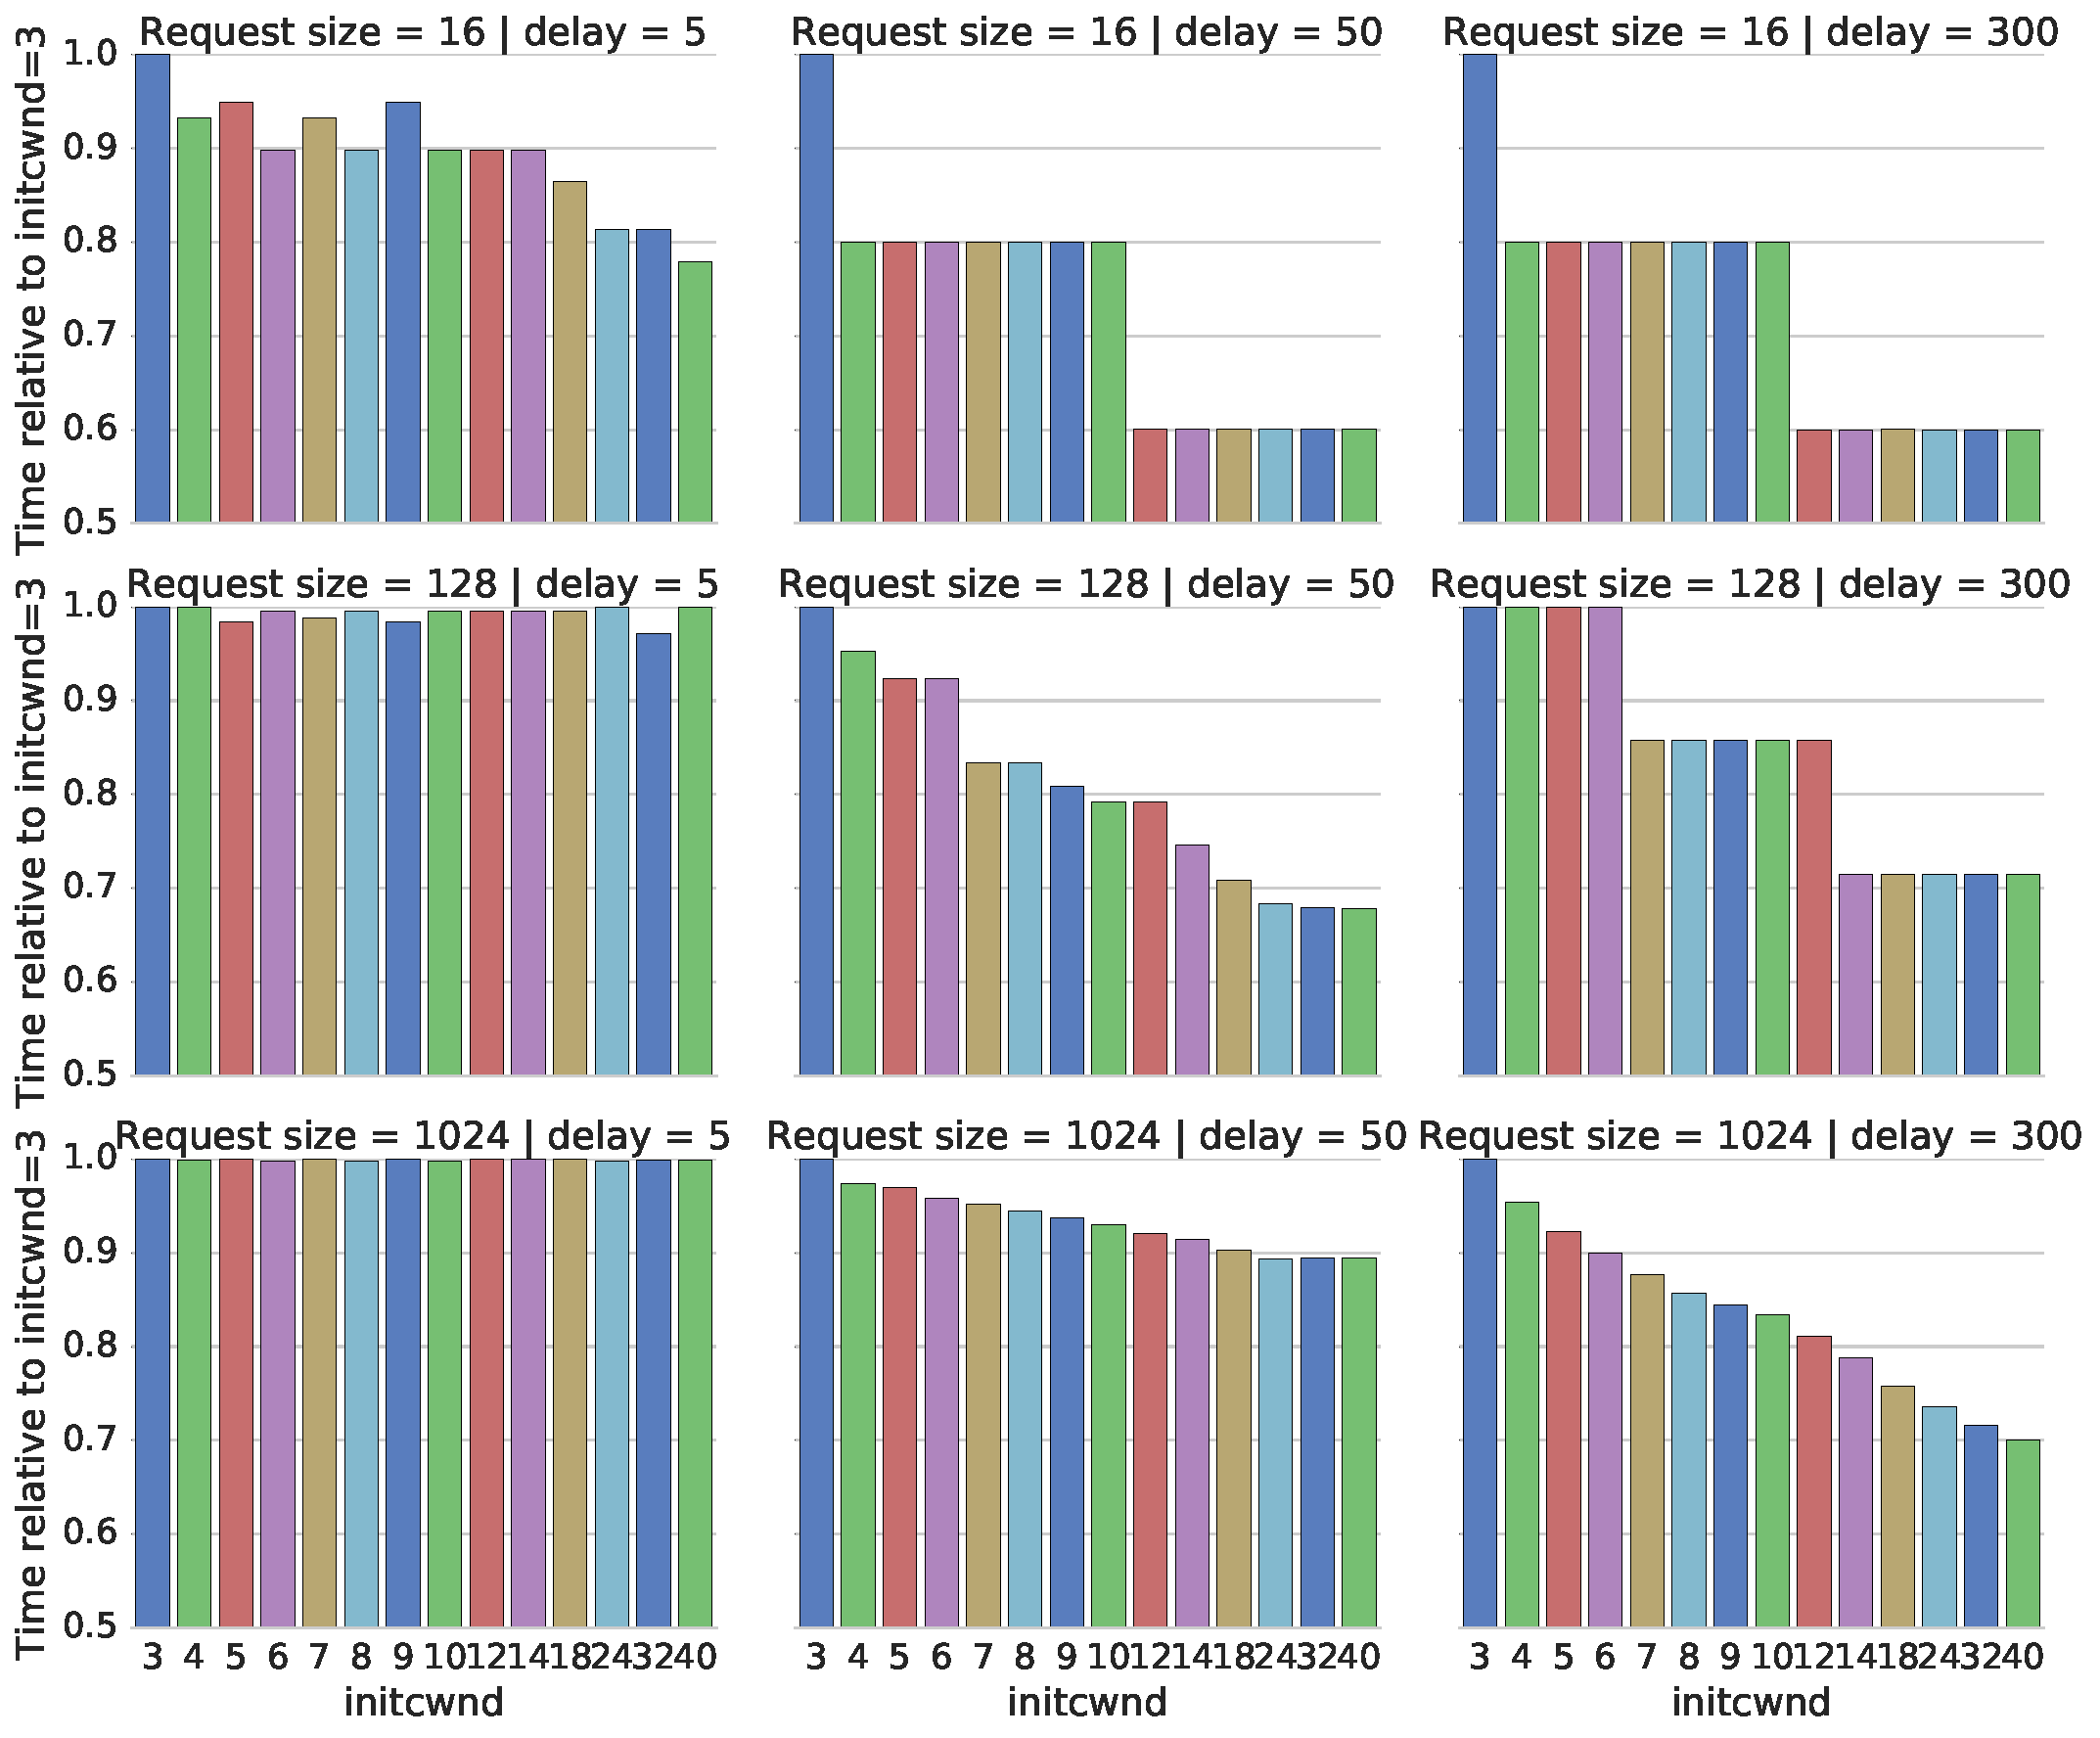
\includegraphics[scale=0.35]{figure/bandwidth-5mb}
\caption{Request time relative to a window of 3 segments with a bandwidth of
5MBps with varying forwarding delay [seconds] and varying request size [kiB]}
\label{fig:bandwith-5mb}
\end{center}
\end{figure*}

\begin{figure*}[ht]
\begin{center}
\footnotesize
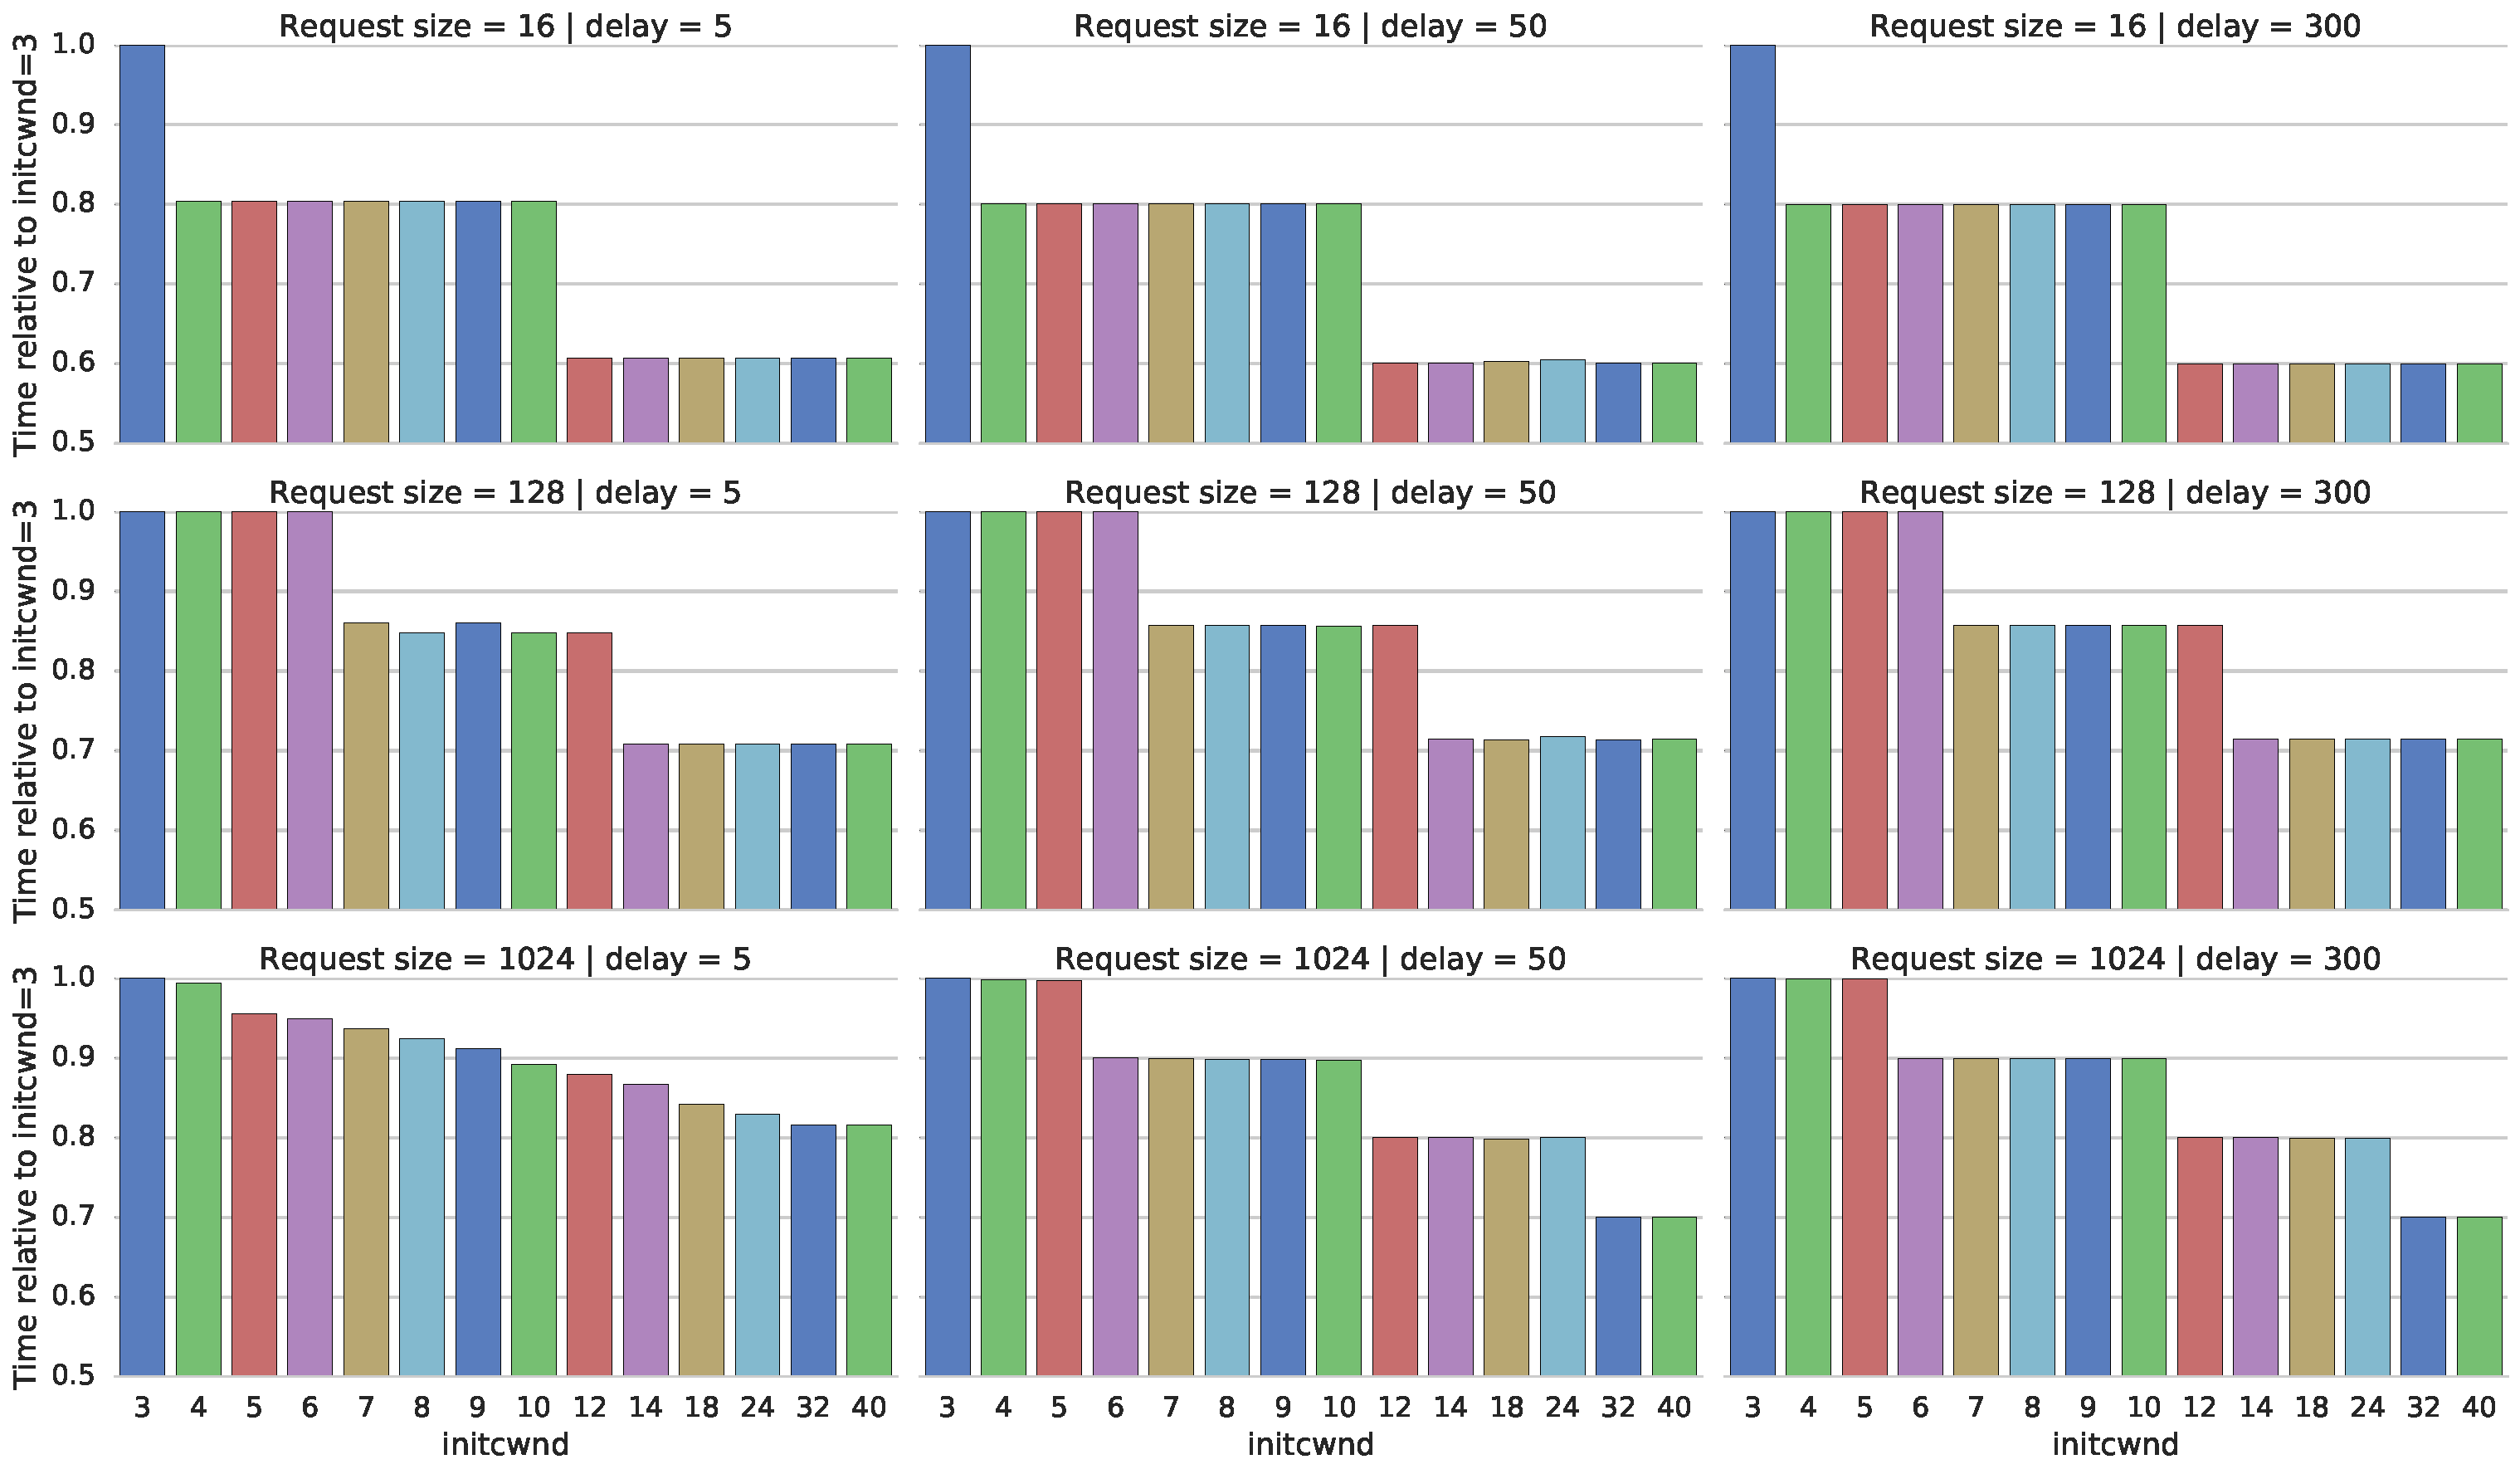
\includegraphics[scale=0.35]{figure/bandwidth-100mb}
\caption{Request time relative to a window of 3 segments with a bandwidth of
100MBps with varying forwarding delay [seconds] and varying request size [kiB]}
\label{fig:bandwith-100mb}
\end{center}
\end{figure*}


\section{Related Work}
\label{sec:related}

\myparagraph{Paper xzy} ?


\section{Conclusion}
\label{sec:conclusion}


%\vspace{-3mm}
\footnotesize
\bibliographystyle{abbrv}

\bibliography{main}
%\appendix


\end{document}
